\documentclass[border=10pt]{standalone}

\usepackage{tikz}
\usepackage{tikzsymbols}
\usetikzlibrary{calc,patterns,shapes.geometric}

\def\centerarc[#1](#2)(#3:#4:#5){\draw[#1] ($(#2)+({#5*cos(#3)},{#5*sin(#3)})$) arc (#3:#4:#5);}

\begin{document}
	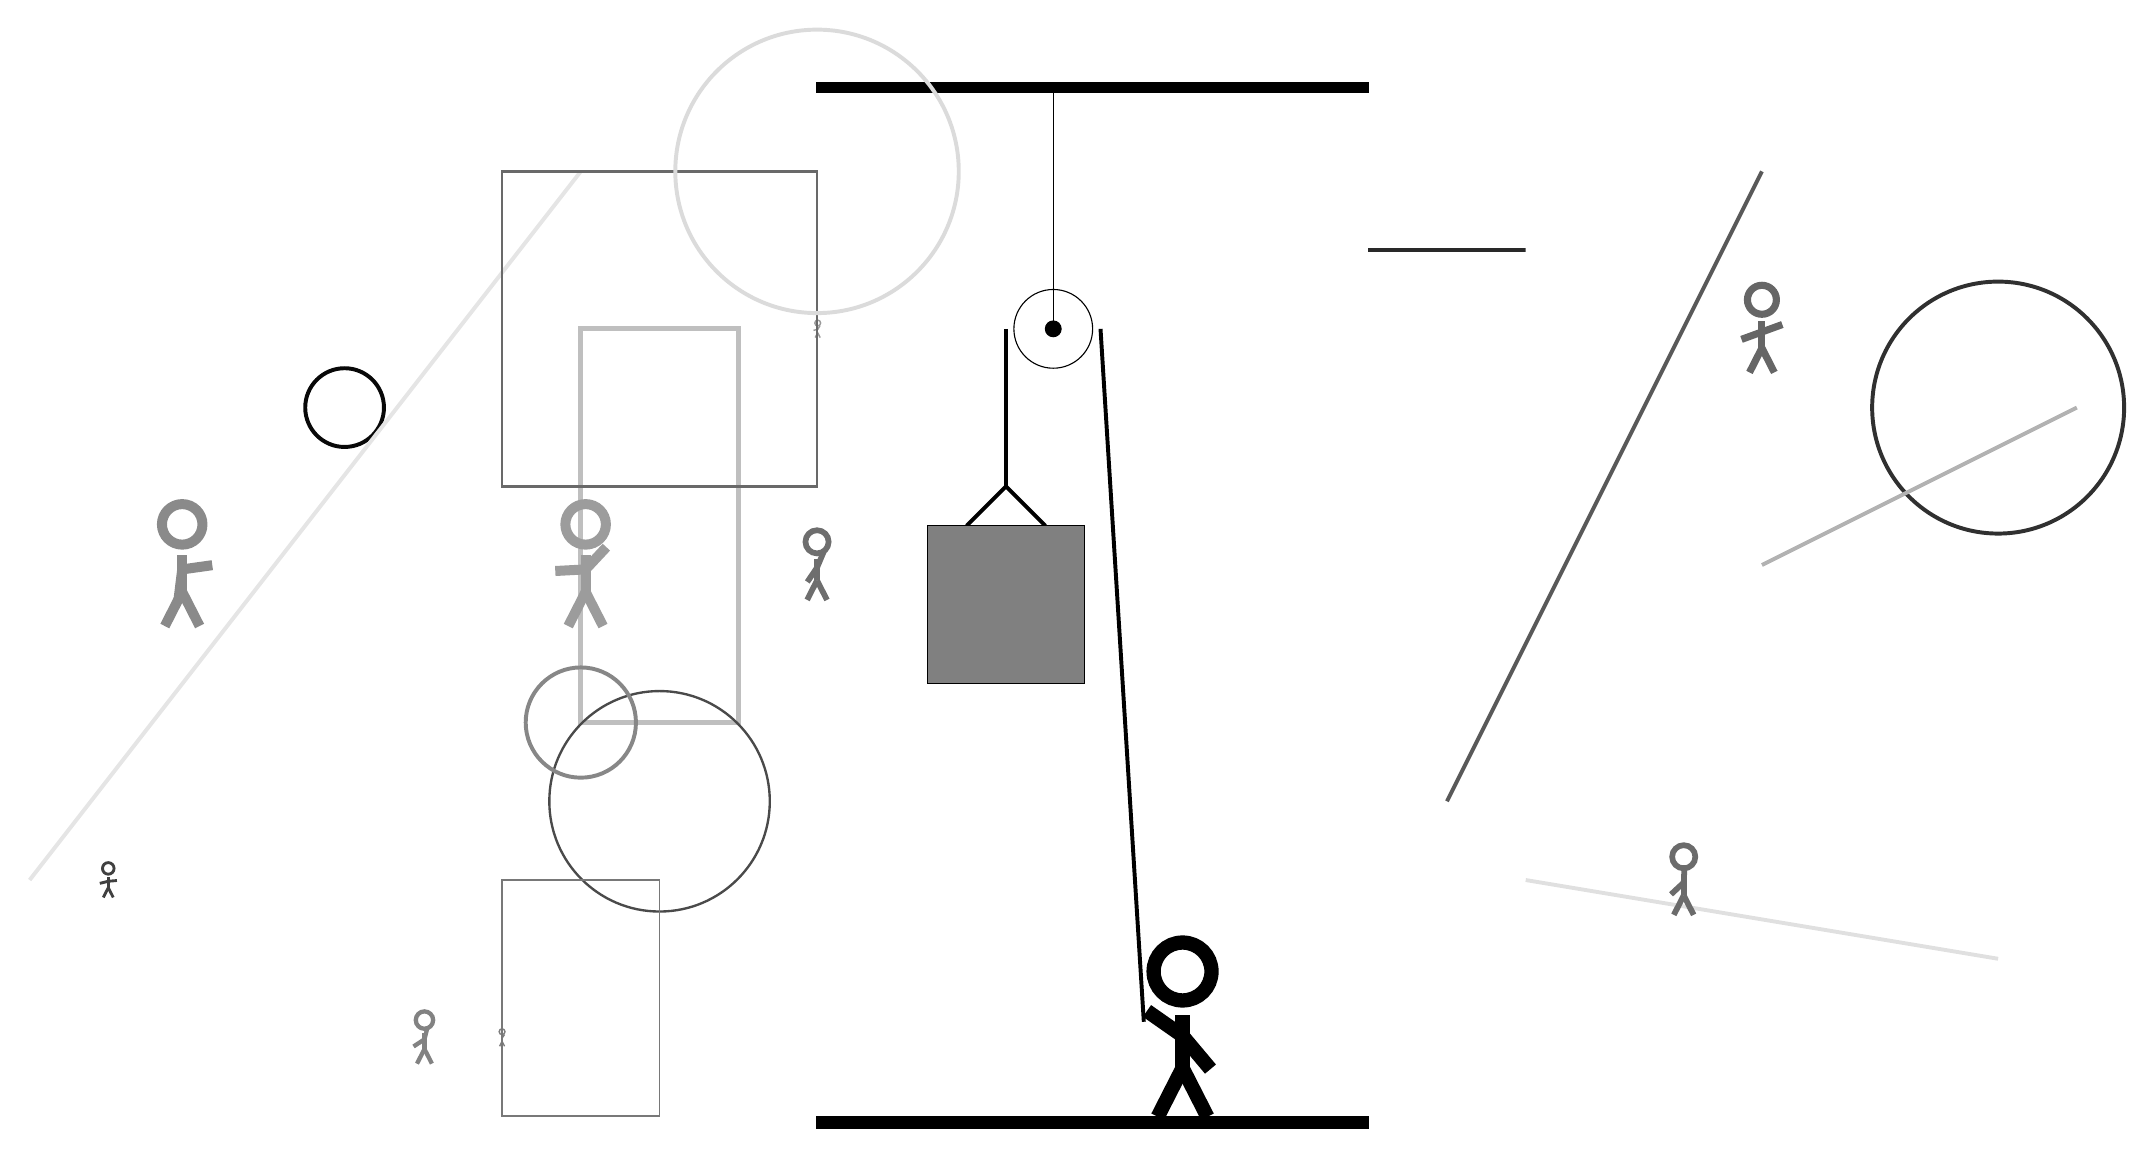
\begin{tikzpicture}
		%%%%% START %%%%%
		
		\draw[fill=black] (-2, 10) rectangle (5, 10.125);
		
		\node[line width=0.5mm, color=black!51] at (-6, -2) {\Strichmaxerl[1][85][56]};
		
		\node[line width=0.2mm, color=black!75] at (-11, 0) {\Strichmaxerl[2][14][5]};
		\draw[line width=0.6mm, color=black!25] (-3, 7) rectangle (-5, 2);
		\draw [line width=0.5mm, color=black!97](-8, 6) circle (0.5);
		
		\draw[line width=0.5mm, color=black!65](6, 1) -- (10, 9);
		
		\draw [line width=0.5mm, color=black!75](-8, -2) circle (0.0);
		\draw[line width=0.5mm, color=black!10](-5, 9) -- (-12, 0);
		
		\node[line width=0.3mm, color=black!40] at (-2, 7) {\Strichmaxerl[1][11][59]};
		\node[line width=0.3mm, color=black!60] at (10, 7) {\Strichmaxerl[5][20][20]};
		\draw[line width=0.3mm, color=black!59] (-2, 9) rectangle (-6, 5);
		\draw[line width=0.5mm, color=black!12](7, 0) -- (13, -1);
		\node[line width=0.3mm, color=black!58] at (9, 0) {\Strichmaxerl[4][43][87]};
		\draw [line width=0.5mm, color=black!81](13, 6) circle (1.6);
		\draw [line width=0.5mm, color=black!14](-2, 9) circle (1.8);
		\draw[line width=0.5mm, color=black!30](10, 4) -- (14, 6);
		\draw [line width=0.3mm, color=black!71](-4, 1) circle (1.4);
		
		\node[line width=0.6mm, color=black!49] at (-7, -2) {\Strichmaxerl[3][33][76]};
		\node[line width=0.2mm, color=black!46] at (-10, 4) {\Strichmaxerl[7][83][8]};
		\draw[line width=0.2mm, color=black!53] (-4, 0) rectangle (-6, -3);
		\draw[line width=0.5mm, color=black!84] (7, 8) rectangle (5, 8);
		\node[line width=0.6mm, color=black!57] at (-2, 4) {\Strichmaxerl[4][56][67]};
		\draw [line width=0.5mm, color=black!47](-5, 2) circle (0.7);
		
		\node[line width=0.5mm, color=black!39] at (-5, 4) {\Strichmaxerl[7][3][47]};
		
		\draw (1, 7) circle (0.5);
		\draw[fill=black] (1, 7) circle (0.1);
		\draw (1, 10) -- (1, 7);
		
		\draw[line width=0.5mm] (-0.1, 4.5) -- (0.4, 5.0) -- (0.9, 4.5);
		\draw[fill=black!50] (-0.6, 4.5) rectangle (1.4, 2.5);
		
		\draw[line width=0.5mm] (0.4, 7) -- (0.4, 5.0);
		\centerarc[line width=0.5mm](1, 7)(0:180:0.6);
		\draw[line width=0.5mm](1.6, 7) -- (2.15, -1.8);
		
		\node at (2.6, -1.9) {\Strichmaxerl[10][-35][-50]};
		
		\draw[fill=black] (-2, -3) rectangle (5, -3.15);
		
		%%%%% END %%%%%
	\end{tikzpicture}
\end{document}